%!TEX TS-program = pdflatex
%!TEX root = tesi.tex
%!TEX encoding = UTF-8 Unicode

\chapter{Conclusioni}
% TODO recap chapter?

\section{Commento Sui Risultati}\todo[noline]{scegliere titolo migliore}
Innanzitutto è bisognoso confrontare i risultati ottenuti con gli obbiettivi posti all'inizio di questo documento.
Si ricorda che uno dei principali obbiettivi era non scartare più del 2\% dei Conformi.
Osservando i risultati ottenuti si può vedere che, nonostante i numeri con cui le percentuali sono state calcolate siano piuttosto piccoli, nessun Conforme dell'insieme di \textit{test} è stato classificato in modo scorretto.
Questo significa una quantità di Falsi Positivi pari allo 0\%.
Verificando le capacità del sistema anche sull'insieme d'allenamento, risulta che lo 1.1\% di elementi è stato classificato come Scarto, principalmente foto scattate ad una distanza superiore alla media.

Identificare il maggior numero possibile di elementi della classe Scarto, idealmente tutti.
Va fatto notare che difficilmente un sistema è perfetto, infatti di solito richiedere un'alta capacità di riconoscimento per una classe porta ad un calo di accuratezza per un'altra.
%Intuitivamente 
Quindi l'avere come obbiettivo un sistema che lasci passare tutti i Conformi e allo stesso tempo sia chirurgico nell'identificazione degli Scarti significa porsi di fronte ad una sfida notevole.
L'inseme di algoritmi descritto in questo documento identifica uno Scarto con un'accuratezza del 93.3\%.
Purtroppo il numero limitato di campioni per questa classe non ci permette di tracciare delle percentuali che possano definirsi accurate, infatti quel 6.7\% è rappresentato da quattro carcasse appena.
Dopo aver verificato che queste quattro carcasse presentano colle con caratteristiche simili, non possiamo dire con sicurezza quale sia la frequenza di creazione di quei particolari tipi di colla (di forma molto sottile ed allungata).
Si suppone però che gli esemplari Scarto a nostra disposizione catturino sufficientemente bene la forma più frequente di colla, concludiamo che questo risultato sia soddisfacente.

Bisogna fare un'ultima considerazione sulla adattabilità e flessibilità della soluzione proposta.
Poiché entrambi gli algoritmi di \textit{pre} e \textit{post-processing} sono stati creati ed impostati manualmente hanno flessibilità ridotta.
È possibile che, al variare della calibratura del processo di raccolta immagini, si ottengano risultati inaspettati.
Basti pensare che le dimensioni della maschera applicata in fase di \textit{pre-processing} non sono adattative, ciò significa che ad esempio, al variare della distanza della fotocamere dal fondo della carcassa, non possiamo esser certi né che tutti i gradini siano visibili né che le balze vengano nascoste completamente.
Infatti proprio quest'ultimo è il principale motivo di classificazione errata di alcuni Conformi: l'incapacità del primo algoritmo di nascondere correttamente le balze della carcassa.
Va però fatto notare che sono algoritmi facilmente modificabili e che la loro calibratura potrebbe essere effettuata durante la calibratura del macchinario, dato che il risultato dipende da pochi parametri.

Per quanto riguarda l'\textit{autoencoder} si può dire che il suo allenamento è rapido e richiede un numero esiguo di risorse.
Soprattutto non è richiesto che il \textit{dataset} sia etichettato a mano, pratica dispendiosa e prona ad errori.
Inoltre, anche qualora l'inseme di immagini contenesse elementi della classe errata, ciò non sarebbe un problema.
Queste caratteristiche permettono di creare nuovi \textit{dataset} in un tempo molto ridotto rispetto ad altre tecniche.

\section{Soluzione Alternativa}
Una soluzione alternativa che merita \todo{forse dire meglio} sicuramente almeno un commento riguarda la segmentazione semantica e più nello specifico le U-Net~\cite{unet}.
La segmentazione permette di associare ad ogni \textit{pixel} di un'immagine una specifica classe.
Oggi viene usata nei sistemi di guida autonoma perché permette di identificare e distinguere con precisione la carreggiata, gli eventuali ostacoli, le altre macchine e soprattutto i pedoni e la segnaletica stradale.
Le reti neurali utilizzate per questo compito vengono chiamate U-Net a causa della loro architettura che, come si vede in figura~\ref{fig:unet}, ricorda la forma di una U.
Queste reti hanno una struttura simile agli \textit{autoencoder} perché si possono distinguere una fase discendete ed una di risalita.
Ma ci sono due principali differenze:
\begin{enumerate}
  \item si vuole mantenere più informazione possibile.
    Ciò viene effettuato raddoppiando il numero di canali in corrispondenza di ogni \textit{max-pooling layer}.

  \item in corrispondenza di layer con la stessa dimensione $n$ vengono effettuati dei TODO e si appiccica le feature in coda \todo{leggere paper per terminologia}.

\end{enumerate}
Le U-Net vengono allenate per fornire in \textit{output} un'immagine in cui aree di \textit{pixel} sono colorate con il colore della classe corrispondente.
Sia $I$ l'immagine in ingresso e sia $L$ una copia di $I$ in cui ogni elemento è stato colorato a mano con il colore della relativa classe.
Durante l'allenamento si vuole minimizzare la differenza tra l'immagine $L'$ creata dalla rete e la $L$ fornita.
In questo modo il modello è spinto a creare delle relazioni tra ciò che è rappresentato nell'immagine in ingresso ed i colori attesi in uscita.

\begin{figure}[ht]
  \begin{center}
    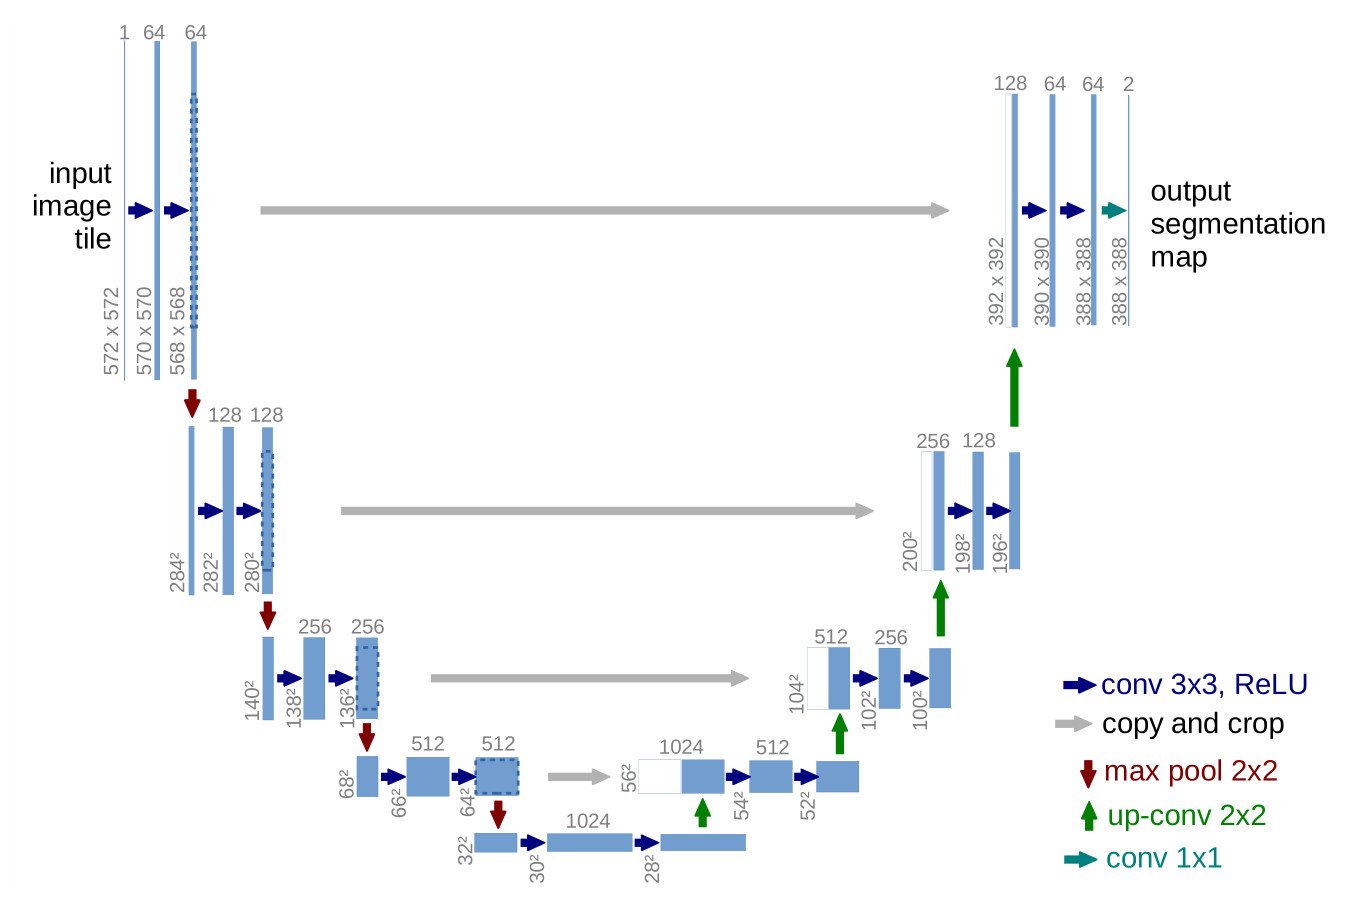
\includegraphics[width=\textwidth]{unet}
    \caption{Architettura di una U-Net}
    \label{fig:unet}
  \end{center}
\end{figure}

Nel nostro caso il problema di segmentazione, riconosciuto universalmente come un problema di grande complessità, viene semplificato notevolmente: si vuole riconoscere soltanto i \textit{pixel} relativi alla colla.
Quindi verranno usati soltanto due colori, uno sarà associato alla colla, mentre il secondo a tutto ciò che non è colla.
Il principale problema di 


